\documentclass{article}
\usepackage{graphicx}
\usepackage{myTitle}
\usepackage{amsthm}
\usepackage{amssymb}
\usepackage{amsmath}
\usepackage[bb=boondox]{mathalfa}
\usepackage[utf8]{inputenc}
\usepackage[T1]{fontenc}
\usepackage[french]{babel}

\newtheorem{theorem}{Théorème}[section]
\newtheorem{corollary}{Corollaire}[theorem]
\newtheorem{lemma}[theorem]{Lemme}

\theoremstyle{definition}
\newtheorem{definition}{Définition}[section]

\theoremstyle{remark}
\newtheorem*{remark}{Remarque}
\newtheorem*{note}{Note}
\newtheorem*{example}{Exemple}

%\begin{claim}
%\begin{proposition}
%\begin{conjecture}
%\begin{observation}

\begin{document}

\title{Jeux, Synthèses et Contrôles}
\subtitle{\large Cours 3 : Agnostic setting}
\prof{Nathanaël FIJALKOW}
\author{CARN, Zahra} %\and
\date{Thursday 8 October 2020}

\maketitle

\tableofcontents
\newpage

\section{Inégalités utiles à savoir}
\begin{equation}
    e^x\geq 1+x, \quad x\in\mathbb{R}
\end{equation}
\begin{equation}
    (1+x)^a\geq 1+xa, \quad a,x\geq 0
\end{equation}
\begin{equation}\tag{Union Bound}
    \mathbb{P}(A\cup B)\leq\mathbb{P}(A)+\mathbb{P}(B)
\end{equation}

\section{Agnostic Setting}

En français : modèle agnostique\\

$\begin{array}{c|l}
    \mbox{\textbf{modèle}} & X,Y\quad \mathcal{H} \mbox{ ensemble de fonctions } X\to Y \\
    \hline
    \mbox{consistant} & \mbox{On suppose }\exists c\in\mathcal{H} \mbox{ et le sample } S=\{(x_i,c(x_i))\}_i\\
    & \mbox{Objectif : Trouver } h\in\mathcal{H} \mbox{ cohérent avec } S\\
    \hline
    \mbox{PAC} & \mbox{On suppose } \mathcal{D}\mbox{ sur } X, \exists c\in\mathcal{H} \mbox{ et } S\sim\mathcal{D}^m, S=\{(x_i,c(x_i))\}_i\\
    & \mbox{Objectif : } \mathbb{P}_{S\sim\mathcal{D}^m}(\mbox{err}_c(h)\leq\epsilon )\geq 1-\delta \\
    & \mbox{ où } \mbox{err}_c(h)=\mathbb{P}_{x\sim\mathcal{D}}(h(x)\neq c(x))\\
    \hline
    %
    \mbox{agnostic PAC} & \mbox{On suppose } \mathcal{D}\mbox{ sur } X\times Y, S\sim\mathcal{D}^m, S=\{(x_i,y_i)\}_i\\
    & \mbox{err}(h)= \mathbb{P}_{(x,y)\sim\mathcal{D}} (h(x)\neq y)\\
    & \mbox{Objectif : } \mathbb{P}_{S\sim\mathcal{D}^m}(\mbox{err}(h)-\mbox{inf}_{h'\in\mathcal{H}}\mbox{err}(h')\leq\epsilon)\geq 1-\delta\\
\end{array}$

On note que $\mbox{inf}_{h'\in\mathcal{H}}\mbox{err}(h')$  le modèle  agnostic PAC prend en quelque sorte le rôle de $c\in\mathcal{H}$ dans le modèle PAC. 

\begin{definition}[Erreur empirique]
    $$h\in\mathcal{H}, \widehat{\mbox{err}}(h) = \widehat{\mbox{err}}(h)=\frac{1}{m}\Sigma_{i=1}^m\mathbb{1}_{h(x_i)\neq y_i}$$
\end{definition}

\begin{note}
    $\mathbb{1}$ est la fonction indice défini par 
    $\mathbb{1}_{A} =
        \begin{cases}
            1 & \text{si $A$}\\
            0 & \text{sinon}
        \end{cases}
    $
\end{note}
\begin{note}  
    $\widehat{}$  est utilisé en probabilités et statistiques pour représenter une valeur \textbf{empirique}. C'est à dire une valeur qui est calculée à partir de données. 
\end{note}
\begin{note}
    $\mbox{arg min}_{x\in X} f(x)$ retourne une valeur $x_{min}\in X$ tel que $f(x_{min}) = \mbox{min}_{x\in X} f(x)$.  
\end{note}

\begin{definition}[ERM]
    $h$ est une hypothèse ERM (\textit{empirical risk minimisation}) si $h = \mbox{arg min}_{h'\in\mathcal{H}}\widehat{\mbox{err}}(h')$.
\end{definition}

Un algorithme ERM retourne $h$ ERM.

$\mathcal{H}$ est apprenable au sens agnostic PAC s'il existe un algo : 
\begin{multline}
    \forall\epsilon, \forall S, \forall\mathcal{D} \mbox{ sur } X\times Y, \exists M\in\mathbb{N}, \forall m\geq M, \\
    \mathcal{P}_{S\sim\mathcal{D}^m}(\mbox{err}(h)-\mbox{inf}_{h'\in\mathcal{H}}\mbox{err}(h')\leq\epsilon)\geq 1-\delta
\end{multline}

%$\vec{a}$

\begin{theorem}
    $\mathcal{H}$ est apprenable au sens agnostic PAC si et seulement si $\mathcal{H}$ a VC dimension ($VCdim$) fini. 
\end{theorem}
\textit{Cette théorème sera prouvé au cours 4.}

\begin{definition}[UCP]
    Propriété de convergence uniforme (\textit{uniform convergence property}) avec un $\epsilon$ fixé
    
    $\forall h\in\mathcal{H}, |\mbox{err}(h)-\widehat{\mbox{err}}(h)|\leq\frac{\epsilon}{2}$
    avec $\mbox{err}(h) = \mathbb{P}_{(x,y)\in\mathcal{D}}(h(x)\neq y)$
\end{definition}
Cette définition permet de simplifier l'objectif de agnostic PAC. 

\begin{lemma}
    On note $h_{ERM}$ une hypothèse ERM tel que $\widehat{\mbox{err}}(h_{ERM})=\mbox{min}_{h\in\mathcal{H}}\widehat{\mbox{err}}(h)$

    Si UCP est vrai (pour $\epsilon$ fixé), alors l'algorithme ERM satisfait $$\mbox{err}(h_{ERM}) - \mbox{inf}_{h\in\mathcal{H}}\mbox{err}(h)\leq\epsilon$$
\end{lemma}

\begin{proof}
    Notons $\mbox{err}(h_{OPT})=\mbox{inf}_{h\in\mathcal{H}}\mbox{err}(h) \Leftrightarrow h_{OPT}=\mbox{arg inf}_{h\in\mathcal{H}}\mbox{err}(h)$
    
    Objectif : Montrer que $\mbox{err}(h_{ERM})-\mbox{err}(h_{OPT})\leq\epsilon$.
    
    On a 
    \begin{align*}
        \mbox{err}(h_{ERM})-\mbox{err}(h_{OPT}) &= \mbox{err}(h_{ERM})-\widehat{\mbox{err}}(h_{ERM})+\widehat{\mbox{err}}(h_{ERM})-\mbox{err}(h_{OPT})\\
        &\hspace{5em} \leq\frac{\epsilon}{2}\mbox{ UCP }
        \hspace{3em} \leq\widehat{\mbox{err}}(h_{OPT})\mbox{ par définition}\\
        &\leq \frac{\epsilon}{2}+\widehat{\mbox{err}}(h_{OPT})-\mbox{err}(h_{OPT})\\
        &\hspace{7em} \leq\frac{\epsilon}{2}\mbox{ UCP}\\
        &\leq \epsilon
    \end{align*}
\end{proof}

$$X, Y={0,1}, S\subseteq X$$

$\mathcal{H}$ ensemble de fonctions $X\to {0,1}$ correspond à un ensemble de sous-ensembles de $X$.

\begin{definition}
    $S$ est \textit{shattered} ("explosé" en français) par $\mathcal{H}$ si
    \begin{equation*}
        \forall P\subseteq S, \exists h\in\mathcal{H}, \forall x\in S, h(x) = 1 \Leftrightarrow x\in P
    \end{equation*}
\end{definition}

\begin{example}
    $X=\mathbb{R}^n, \mathcal{H}_n = \{f | \mathbb{R}^n\to\{0,1\} : f(\vec{x})=
    \begin{cases}
            1 & \text{si } \vec{x}.\vec{a}\geq 0\\
            0 & \text{sinon}
    \end{cases}
    \}
    $\\
    avec $\vec{a}\in\mathbb{R}^n, b\in\mathbb{R}$
    
    $\mathcal{H}_2$ explose $S:=\{(x,y),(x',y')\}$, avec $(x,y), (x',y')\in\mathbb{R}^2$. Une visualisation d'un exemple est donnée dans la figure \ref{fig:cas2}.
    
    \begin{figure}[ht]
        \centering
        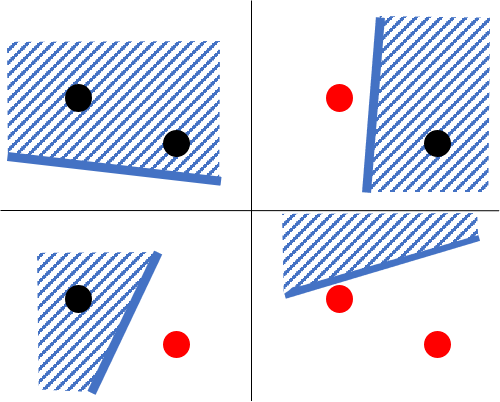
\includegraphics[]{img/h2.png}
        \caption{Visualisation d'une explosion par $\mathcal{H}_2$}
        \label{fig:cas2}
    \end{figure}
    
    $\mathcal{H}_2$ explose $S:=\mbox{3 points non-alignées du plan}$.
    
    $\mathcal{H}_2$ n'explose pas $S:=\mbox{4 points quelconques du plan}$.
\end{example}

\begin{definition}
    $\mbox{VCdim}(\mathcal{H}) = \mbox{max}\{|S|:S \mbox{ explosé par }\mathcal{H}\}$
\end{definition}

\begin{example}[$\mathcal{H}_2$]
    $\mbox{VCdim}(\mathcal{H}_2)=3$ car $\exists S, |S|=3 \mbox{ explosé}$ et $\forall S, |S|\geq 4 \mbox{ non explosé}$
\end{example}

\begin{example}[$\mbox{VCdim}(\mathcal{H})=\infty$]
    $X=\mathbb{N}, \mathcal{H} \mbox{ toutes les fonctions}$
\end{example}

\begin{example}[$\mathcal{H}_n$]
    $\mbox{VCdim}(\mathcal{H}_n)=n+1$
    
    \textit{Une présentation au sujet aura lieu dans quelques semaines.}
\end{example}

\begin{definition}[Fonction de croissance]
    \begin{equation*}
        S\subseteq X, h\in\mathcal{H}, h:X\to\{0,1\},h|_s:S\to\{0,1\}
    \end{equation*}
    
    \begin{equation}
        \Pi_{\mathcal{H}} : \mathbb{N}\to\mathbb{N}\quad\quad m\to\mbox{ max }_{|S|=m, S\subseteq X} |\{h|_S :h\in\mathcal{H}\}|
    \end{equation}
\end{definition}

\begin{example}
    Si $\mbox{VCdim}(\mathcal{H})=d$ que vaut $\Pi_{\mathcal{H}}(d)$ ? $2^d$
    
    Que vaut $\Pi_{\mathcal{H}}(d-1)$ ? $2^m$, pour $m\leq d$
    
    Que vaut $\Pi_{\mathcal{H}}(d+1)$ ? <$2^{d+1}$
\end{example}

\begin{remark}
    $S$ explosé par $\mathcal{H} \Leftrightarrow |\{h|S : h\in\mathcal{H}\}|=2^d$
\end{remark}

\begin{lemma}[Sauer]
    Si $\mbox{VCdim}(\mathcal{H})=d$ alors 
    $$\Pi_{\mathcal{H}}(m)\leq\binom{m}{0}+\binom{m}{1}+...+\binom{m}{d}=\sum_{i=0}^d \binom{m}{i}\leq(\frac{em}{d})^d=O(m^d)$$
\end{lemma}

Les instances de la forme $X$ infini, $\mathcal{H}$ toutes les fonctions $X\to\{0,1\}$ sont impossibles à apprendre.

\textit{Détails à venir}

\end{document}
